%  \documentclass[DIV=12, a4]{scrartcl}
%\documentclass[12pt, a5]{scrartcl}

% \documentclass[a4paper]{report}
% \usepackage[
% % fancytheorems, 
% noindent, 
% %spacingfix, 
% %noheader
% ]{vanilla}


\documentclass[a4paper]{scrreprt}
\usepackage[
fancytheorems, 
noindent, 
% %spacingfix, 
% %noheader,
fancyproofs
]{adam} 

\usepackage{tikz}
\usepackage{asymptote}
\usepackage{cancel}

% \usepackage{subfig}

\setcounter{chapter}{-1}

\title{Vector Calculus}
% \subtitle{Adam Kelly}
\author{Adam Kelly}
% \date{Michaelmas 2020}
\date{\today}

\begin{document}

\maketitle

\begin{abstract}
	This set of notes is a work-in-progress account of the course `Vector Calculus', originally lectured by Dr Anthony Ashton in Lent 2020 at Cambridge. These notes are not a transcription of the lectures, but they do roughly follow what was lectured (in content and in structure).

	These notes are my own view of what was taught, and should be somewhat of a superset of what was actually taught. I frequently provide different explanations, proofs, examples, and so on in areas where I feel they are helpful. Because of this, this work is likely to contain errors, which you may assume are my own. If you spot any or have any other feedback, I can be contacted at \href{mailto:ak2316@cam.ac.uk}{ak2316@cam.ac.uk}.
\end{abstract}

\tableofcontents

\clearpage
\chapter{Introduction}



% \section{Structure of the Course}

% This course is, quite naturally, divided into three sections.

% \begin{enumerate}
% 	\item \emph{Groups}
	
% 	We will be continuing on from IA Groups, paying particular attention to certain topics such as simple groups, $p$-groups and $p$-subgroups. The main highlight of this part of the course will be the Sylow theorems.

% 	\item \emph{Rings}
	
% 	Rings are sets where we can add, subtract and multiply (but not necessarily divide), for example, $\Z$. A ring where division is always possible is a field, for example $\Q$, $\R$ and $\Z/p\Z$ for a prime $p$.

% 	\item \emph{Modules}
	
% 	A module is the analog of a vector space where we work over a ring, rather than a field. We will attempt to classify modules over certain `nice' rings. This will allow us to prove the Jordan Normal theorem of matrices and to classify finite abelian groups. 
% \end{enumerate}

% \section{Books}
% ese books in either your college library or the university library.


\section{Notation}

Throughout this course, a column vector
$$
\begin{pmatrix}
a \\ b\\ c
\end{pmatrix}
$$
is to be interpreted as the vector $\vv{x} = a \vv{e}_x + b \vv{e}_y + c\vv{e}_z$, where $\{\vv{e}_x, \vv{e}_y, \vv{e}_z\}$ are basis vectors aligned with the fixed Cartesian $x$, $y$ and $z$ axes in $\R^3$.

\begin{center}
    \begin{tikzpicture}
        \draw [->,>=stealth] (0, 0) -- (0, 2) node [anchor=south] {$\vv{e}_y$};
        \draw [->,>=stealth] (0, 0) -- (1.95, -0.4) node [anchor=west] {$\vv{e}_x$};
        \draw [->,>=stealth] (0, 0) -- (-1.45, -1) node [anchor=north east] {$\vv{e}_z$};
    \end{tikzpicture}
\end{center}

We may also use the notation $\vv{e}_1 = \vv{e}_x$, $\vv{e}_2 = \vv{e}_y$ and $\vv{e}_3 = \vv{e}_z$, and then we can write $\vv{x} = x_i \vv{e}_i$.

We will also be using the summation convention frequently, which you can read more about in the `Vectors and Matrices' course notes.

\clearpage


\chapter{Differential Geometry of Curves}

We will begin by studying the differential geometry of curves in $\R^3$, which sounds exciting but isn't.

\section{Parameterized Curves \& Arc Length}

The first object we shall study is \emph{parameterized curves}.

\begin{definition}[Parameterized Curve]
	A \vocab{parameterized curve} $C$ in $\R^3$ is the image of a continuous map $\vv{x} : [a, b] \rightarrow \R^3$ in which $t \mapsto \vv{x}(t)$.
\end{definition}

In Cartesian coordinates, we can write
$$
\vv{x}(t) = \begin{pmatrix}
	x_1 (t) \\
	x_2 (t) \\
	x_3(t)
\end{pmatrix} = \begin{pmatrix}
	x (t) \\
	y (t) \\
	z (t)
\end{pmatrix}.
$$

We also give the curve an orientation, based on the map going from the image of $A$ to the image of $B$.

\begin{center}
	


	\tikzset{every picture/.style={line width=0.75pt}} %set default line width to 0.75pt        

	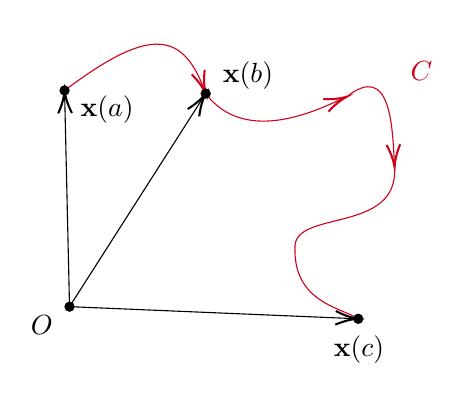
\begin{tikzpicture}[x=0.75pt,y=0.75pt,yscale=-1,xscale=1]
	%uncomment if require: \path (0,300); %set diagram left start at 0, and has height of 300
	
	%Curve Lines [id:da3276060381490892] 
	\draw [color={rgb, 255:red, 208; green, 2; blue, 27 }  ,draw opacity=1 ]   (176,103.75) .. controls (195.37,129.27) and (231.27,111.02) .. (242.33,105.98) ;
	\draw [shift={(244,105.25)}, rotate = 517.62] [color={rgb, 255:red, 208; green, 2; blue, 27 }  ,draw opacity=1 ][line width=0.75]    (10.93,-3.29) .. controls (6.95,-1.4) and (3.31,-0.3) .. (0,0) .. controls (3.31,0.3) and (6.95,1.4) .. (10.93,3.29)   ;
	%Curve Lines [id:da867110150451944] 
	\draw [color={rgb, 255:red, 208; green, 2; blue, 27 }  ,draw opacity=1 ]   (244,105.25) .. controls (264.86,88.76) and (265.95,118.37) .. (266.91,137.51) ;
	\draw [shift={(267,139.25)}, rotate = 266.99] [color={rgb, 255:red, 208; green, 2; blue, 27 }  ,draw opacity=1 ][line width=0.75]    (10.93,-3.29) .. controls (6.95,-1.4) and (3.31,-0.3) .. (0,0) .. controls (3.31,0.3) and (6.95,1.4) .. (10.93,3.29)   ;
	%Curve Lines [id:da48281776098084617] 
	\draw [color={rgb, 255:red, 208; green, 2; blue, 27 }  ,draw opacity=1 ]   (267,139.25) .. controls (269,171.75) and (218,159.25) .. (219,178.25) .. controls (218.5,204.25) and (241,206.75) .. (249.5,212.25) ;
	%Shape: Circle [id:dp01912153166389552] 
	\draw  [draw opacity=0][fill={rgb, 255:red, 0; green, 0; blue, 0 }  ,fill opacity=1 ] (107.9,206.4) .. controls (107.9,205.02) and (109.02,203.9) .. (110.4,203.9) .. controls (111.78,203.9) and (112.9,205.02) .. (112.9,206.4) .. controls (112.9,207.78) and (111.78,208.9) .. (110.4,208.9) .. controls (109.02,208.9) and (107.9,207.78) .. (107.9,206.4) -- cycle ;
	%Curve Lines [id:da9083644795099863] 
	\draw [color={rgb, 255:red, 208; green, 2; blue, 27 }  ,draw opacity=1 ]   (108,102.25) .. controls (147.2,72.85) and (164.31,72.26) .. (175.33,101.9) ;
	\draw [shift={(176,103.75)}, rotate = 250.75] [color={rgb, 255:red, 208; green, 2; blue, 27 }  ,draw opacity=1 ][line width=0.75]    (10.93,-3.29) .. controls (6.95,-1.4) and (3.31,-0.3) .. (0,0) .. controls (3.31,0.3) and (6.95,1.4) .. (10.93,3.29)   ;
	%Shape: Circle [id:dp4960073350824441] 
	\draw  [draw opacity=0][fill={rgb, 255:red, 0; green, 0; blue, 0 }  ,fill opacity=1 ] (105.5,102.25) .. controls (105.5,100.87) and (106.62,99.75) .. (108,99.75) .. controls (109.38,99.75) and (110.5,100.87) .. (110.5,102.25) .. controls (110.5,103.63) and (109.38,104.75) .. (108,104.75) .. controls (106.62,104.75) and (105.5,103.63) .. (105.5,102.25) -- cycle ;
	%Shape: Circle [id:dp8712280703593382] 
	\draw  [draw opacity=0][fill={rgb, 255:red, 0; green, 0; blue, 0 }  ,fill opacity=1 ] (173.5,103.75) .. controls (173.5,102.37) and (174.62,101.25) .. (176,101.25) .. controls (177.38,101.25) and (178.5,102.37) .. (178.5,103.75) .. controls (178.5,105.13) and (177.38,106.25) .. (176,106.25) .. controls (174.62,106.25) and (173.5,105.13) .. (173.5,103.75) -- cycle ;
	%Shape: Circle [id:dp9346879620682326] 
	\draw  [draw opacity=0][fill={rgb, 255:red, 0; green, 0; blue, 0 }  ,fill opacity=1 ] (247,212.25) .. controls (247,210.87) and (248.12,209.75) .. (249.5,209.75) .. controls (250.88,209.75) and (252,210.87) .. (252,212.25) .. controls (252,213.63) and (250.88,214.75) .. (249.5,214.75) .. controls (248.12,214.75) and (247,213.63) .. (247,212.25) -- cycle ;
	%Straight Lines [id:da3352312418861193] 
	\draw    (110.4,206.4) -- (247.5,212.17) ;
	\draw [shift={(249.5,212.25)}, rotate = 182.41] [color={rgb, 255:red, 0; green, 0; blue, 0 }  ][line width=0.75]    (10.93,-3.29) .. controls (6.95,-1.4) and (3.31,-0.3) .. (0,0) .. controls (3.31,0.3) and (6.95,1.4) .. (10.93,3.29)   ;
	%Straight Lines [id:da01233126994686784] 
	\draw    (110.4,206.4) -- (174.92,105.44) ;
	\draw [shift={(176,103.75)}, rotate = 482.58] [color={rgb, 255:red, 0; green, 0; blue, 0 }  ][line width=0.75]    (10.93,-3.29) .. controls (6.95,-1.4) and (3.31,-0.3) .. (0,0) .. controls (3.31,0.3) and (6.95,1.4) .. (10.93,3.29)   ;
	%Straight Lines [id:da11748387967404772] 
	\draw    (110.4,206.4) -- (108.05,104.25) ;
	\draw [shift={(108,102.25)}, rotate = 448.68] [color={rgb, 255:red, 0; green, 0; blue, 0 }  ][line width=0.75]    (10.93,-3.29) .. controls (6.95,-1.4) and (3.31,-0.3) .. (0,0) .. controls (3.31,0.3) and (6.95,1.4) .. (10.93,3.29)   ;
	
	% Text Node
	\draw (90.5,209.5) node [anchor=north west][inner sep=0.75pt]    {$O$};
	% Text Node
	\draw (114.5,103.5) node [anchor=north west][inner sep=0.75pt]    {$\mathbf{x}( a)$};
	% Text Node
	\draw (183,87.25) node [anchor=north west][inner sep=0.75pt]    {$\mathbf{x}( b)$};
	% Text Node
	\draw (236.5,219) node [anchor=north west][inner sep=0.75pt]    {$\mathbf{x}( c)$};
	% Text Node
	\draw (273.5,87) node [anchor=north west][inner sep=0.75pt]  [color={rgb, 255:red, 208; green, 2; blue, 27 }  ,opacity=1 ]  {$C$};
	
	
	\end{tikzpicture}

\end{center}

\begin{definition}[Differentiability and Smoothness]
	We say that a curve $C$ is \vocab{differentiable} if each of the components $\{x_1(t), x_2(t), x_3(t) \}$ are differentiable, and say $C$ is \vocab{regular} if $|\vv{x}'(t)| \neq 0$. If $C$ is differentiable and regular then we say $C$ is \vocab{smooth}.
\end{definition}

\begin{remark}
	The `regular' condition exists to avoid `spikes' in the curve. For example, consider the curve $\vv{x}(t) = (t^3, t^2)$. Clearly this is differentiable, but $\vv{x}(t)$ has a cusp at $t = 0$. At $t = 0$, we have $|\vv{x}(0)| = 0$. If this was not the case, there would be no cusp.
\begin{center}
	\begin{asy}
		unitsize(55);
		import graph;
		pair F(real t) {
			return (t^3, t^2);
		}

		path g = graph(F, -1.1, 1.1);

		draw(g, blue + linewidth(0.9pt));

		draw((0, -0.25) -- (0, 1.2), arrow=Arrow(TeXHead));
		draw((-1.3, 0) -- (1.3, 0), arrow=Arrow(TeXHead));
	\end{asy}
\end{center}

\end{remark}


Recall that the function $x_i(t)$ is differentiable at $t$ if $x_i(t + h) = x_i(t) + x_i'(t) h + o(h)$, where $\frac{o(h)}{h} \rightarrow 0$ as $h \rightarrow 0$. We can write this in terms of vectors, where
$$
\vv{x}(t + h) = \vv{x}(t) + \vv{x}'(t)h + o(h),
$$
where $o(h)$ is a vector for which $\frac{|o(h)|}{h} \rightarrow 0$ as $h \rightarrow 0$.
  
Now given some curve $C$, we may want to find the length of the curve. We can try to do this by approximating the curve using straight lines.

\begin{center}
	

\tikzset{every picture/.style={line width=0.75pt}} %set default line width to 0.75pt        

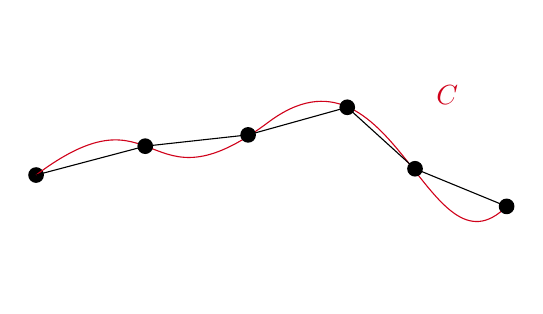
\begin{tikzpicture}[x=0.75pt,y=0.75pt,yscale=-1,xscale=1]
%uncomment if require: \path (0,300); %set diagram left start at 0, and has height of 300

%Shape: Ellipse [id:dp6464695455275871] 
\draw  [draw opacity=0][fill={rgb, 255:red, 0; green, 0; blue, 0 }  ,fill opacity=1 ] (42.5,126.68) .. controls (42.5,124.59) and (44.19,122.9) .. (46.28,122.9) .. controls (48.37,122.9) and (50.06,124.59) .. (50.06,126.68) .. controls (50.06,128.77) and (48.37,130.46) .. (46.28,130.46) .. controls (44.19,130.46) and (42.5,128.77) .. (42.5,126.68) -- cycle ;
%Curve Lines [id:da6916953701818653] 
\draw [color={rgb, 255:red, 208; green, 2; blue, 27 }  ,draw opacity=1 ]   (46.28,126.68) .. controls (106.73,81.34) and (97.66,146.63) .. (158.12,101.29) .. controls (218.57,55.95) and (235.2,179.58) .. (272.98,141.79) ;
%Shape: Circle [id:dp8157615548797015] 
\draw  [draw opacity=0][fill={rgb, 255:red, 0; green, 0; blue, 0 }  ,fill opacity=1 ] (95.09,112.77) .. controls (95.09,110.69) and (96.79,109) .. (98.87,109) .. controls (100.96,109) and (102.65,110.69) .. (102.65,112.77) .. controls (102.65,114.86) and (100.96,116.55) .. (98.87,116.55) .. controls (96.79,116.55) and (95.09,114.86) .. (95.09,112.77) -- cycle ;
%Shape: Ellipse [id:dp6623880161127722] 
\draw  [draw opacity=0][fill={rgb, 255:red, 0; green, 0; blue, 0 }  ,fill opacity=1 ] (144.67,107.33) .. controls (144.67,105.25) and (146.36,103.56) .. (148.45,103.56) .. controls (150.53,103.56) and (152.22,105.25) .. (152.22,107.33) .. controls (152.22,109.42) and (150.53,111.11) .. (148.45,111.11) .. controls (146.36,111.11) and (144.67,109.42) .. (144.67,107.33) -- cycle ;
%Shape: Ellipse [id:dp947023885876757] 
\draw  [draw opacity=0][fill={rgb, 255:red, 0; green, 0; blue, 0 }  ,fill opacity=1 ] (192.43,94.03) .. controls (192.43,91.95) and (194.12,90.26) .. (196.2,90.26) .. controls (198.29,90.26) and (199.98,91.95) .. (199.98,94.03) .. controls (199.98,96.12) and (198.29,97.81) .. (196.2,97.81) .. controls (194.12,97.81) and (192.43,96.12) .. (192.43,94.03) -- cycle ;
%Shape: Ellipse [id:dp9991347478656615] 
\draw  [draw opacity=0][fill={rgb, 255:red, 0; green, 0; blue, 0 }  ,fill opacity=1 ] (225.07,123.66) .. controls (225.07,121.57) and (226.76,119.88) .. (228.85,119.88) .. controls (230.94,119.88) and (232.63,121.57) .. (232.63,123.66) .. controls (232.63,125.74) and (230.94,127.43) .. (228.85,127.43) .. controls (226.76,127.43) and (225.07,125.74) .. (225.07,123.66) -- cycle ;
%Shape: Ellipse [id:dp5868702964474427] 
\draw  [draw opacity=0][fill={rgb, 255:red, 0; green, 0; blue, 0 }  ,fill opacity=1 ] (269.2,141.79) .. controls (269.2,139.71) and (270.89,138.01) .. (272.98,138.01) .. controls (275.07,138.01) and (276.76,139.71) .. (276.76,141.79) .. controls (276.76,143.88) and (275.07,145.57) .. (272.98,145.57) .. controls (270.89,145.57) and (269.2,143.88) .. (269.2,141.79) -- cycle ;
%Straight Lines [id:da7875885498839282] 
\draw    (46.28,126.68) -- (98.87,112.77) ;
%Straight Lines [id:da309124837435779] 
\draw    (98.87,112.77) -- (148.45,107.33) ;
%Straight Lines [id:da8902322155826599] 
\draw    (148.45,107.33) -- (196.2,94.03) ;
%Straight Lines [id:da9085782113625647] 
\draw    (196.2,94.03) -- (228.85,123.66) ;
%Straight Lines [id:da7165214688732946] 
\draw    (228.85,123.66) -- (272.98,141.79) ;

% Text Node
\draw (237.91,82.51) node [anchor=north west][inner sep=0.75pt]  [color={rgb, 255:red, 208; green, 2; blue, 27 }  ,opacity=1 ]  {$C$};


\end{tikzpicture}

\end{center}

For $C:[a, b] \rightarrow \R^3$ with $t \mapsto \vv{x}(t)$, we introduce a partition $P$ of $[a, b]$ with $t_0$, $t_N = b$ and $t_0 < t_1 < \dots < t_N$, and we set $\Delta t_i = t_{i + 1} - t_i$ and $\Delta t = \max_i \Delta t_i$.

\begin{definition}[Length Relative to a Partition]
	For some curve $C$ and partition $P$ as above, we define the \vocab{length} of $C$ relative to $P$ by
	$$
	\ell(C, P) = \sum_{i = 0}^{N - 1} \left|\vv{x}(t_{i + 1}) - \vv{x}(t_i)\right|.
$$
\end{definition}

We would expect that this length would get closer to the true length of $C$ as $\Delta t \rightarrow 0$. Indeed, we will define the length of $C$ in this way.

\begin{definition}[Length of a Curve]
	We define the length of a curve $C$ by
	$$
	\ell(C) = \lim_{\Delta t \to 0} \sum_{i = 0}^{N - 1} \left|\vv{x}(t_{i + 1}) - \vv{x}(t_i) \right| = \lim_{\Delta t \rightarrow 0} \ell(C, P).
	$$
	if this limit does not exist, we say the curve is \vocab{non-rectifiable}.
\end{definition}

In this course, we will not worry too much about non-rectifiable curves, so we will assume that this notion is always well defined.

Now suppose $C$ is a differentiable curve. Then we have that
\begin{align*}
	\vv{x}(t_{i + 1}) &= \vv{x}(t_i + t_{i + 1} - t_i) \\
					&= \vv{x}(t_i + \Delta t_i) \\
					&= \vv{x}(t_i) + \vv{x}'(t_i) \Delta t_i + o(\Delta t_i).
\end{align*}
It follows that
$$
|\vv{x}(t_{i + 1}) - \vv{x}(t_i) | = |\vv{x}'(t_i)| \Delta t_i + o(\Delta t_i). 
$$

So if $C$ is differentiable, we get the expression
$$
\ell(C, P)=\sum_{i=0}^{N-1}\left(\left|\mathbf{x}^{\prime}\left(t_{i}\right)\right| \Delta t_{i}+o\left(\Delta t_{i}\right)\right).
$$
Recall that $o(\Delta t_i)$ represents a function for which $\frac{o(\Delta t_i)}{\Delta t_i} \rightarrow 0$ as $\delta t_i \rightarrow 0$. So for any $\epsilon > 0$, if $\Delta t = \max_i \Delta t_i$  is sufficiently small, then we have
$$
|o(\Delta t_i) | < \left(\frac{\epsilon}{b - a}\right) \Delta t_i,
$$
for $i = \{0, \dots, N - 1\}$. So
\begin{align*}
	\left|\ell(C, P) - \sum_{i = 0}^{N - 1} |\vv{x}' (t_i) \Delta t_i \right| &= \left|\sum_{i = 0}^{N - 1} o(\Delta t_i)\right| \\
	&< \frac{\epsilon}{b - a} \sum_{i = 0}^{N - 1} \Delta{t_i} = \epsilon.
\end{align*}
Thus the LHS tends to zero as $\Delta t \rightarrow 0$. So we get that
\begin{align*}
	\ell(C) &= \lim_{\Delta t \to 0} \ell(C, P) = \lim_{\Delta t \to 0} \sum_{i = 0}^{N - 1} |\vv{x}'(t_i)| \Delta t_i \\
		&= \int_a^b \left|\vv{x}'(t)\right| \; \dd t,
\end{align*}
by the definition of the Riemann integral.
So, we can restate our definition in this other form.

\begin{definition}[Length of a Curve]
	If $C: [a, b] \rightarrow \R^3$ is a differentiable curve with $t \mapsto \vv{x}(t)$, then its \vocab{length} is
	$$
	\ell(C) = \int_a^b |\vv{x}'(t)| \; \dd t = \int_C \dd s,
	$$
where $\dd s$ is the \vocab{arc-length element}, $\dd s = |\vv{x}'(t)| \; \dd t$.
\end{definition}

With this defined, we can define the integral of a function along a curve.

\begin{definition}[Integral on a Curve]
	For a function $f : \R^3 \rightarrow \R$ and a differentiable curve $C: [a, b] \rightarrow \R^3$ with $t \mapsto \vv{x}(t)$, we define the \vocab{integral of $f$ along $C$} to be
	$$
	\int_C f(\vv{x})\; \dd s = \int_a^b f(\vv{x}(t)) |\vv{x}'(t)| \; \dd t.
	$$
\end{definition}

Now consider a curve $C$ made up of $M$ smooth curves $C_1, C_2, \dots, C_M$.

\begin{center}
	

\tikzset{every picture/.style={line width=0.75pt}} %set default line width to 0.75pt        

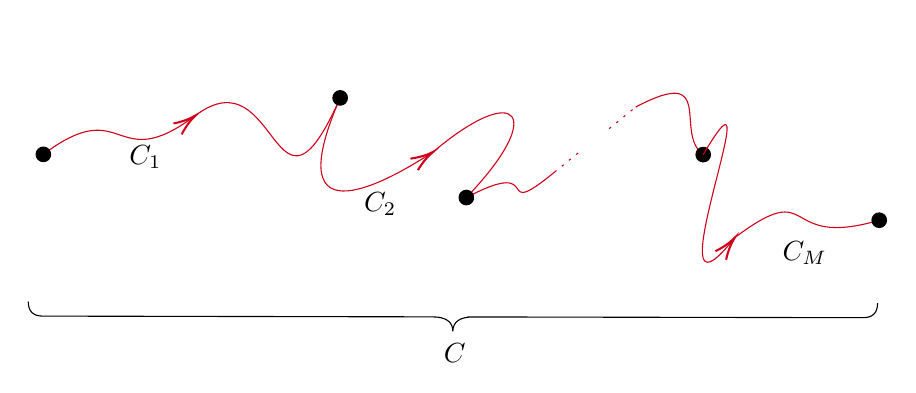
\begin{tikzpicture}[x=0.75pt,y=0.75pt,yscale=-1,xscale=1]
%uncomment if require: \path (0,300); %set diagram left start at 0, and has height of 300

%Curve Lines [id:da5796763237473451] 
\draw [color={rgb, 255:red, 208; green, 2; blue, 27 }  ,draw opacity=1 ]   (37.48,39.48) .. controls (77.08,9.78) and (71.01,49.86) .. (109.69,21.56) ;
\draw [shift={(110.88,20.68)}, rotate = 503.13] [color={rgb, 255:red, 208; green, 2; blue, 27 }  ,draw opacity=1 ][line width=0.75]    (10.93,-3.29) .. controls (6.95,-1.4) and (3.31,-0.3) .. (0,0) .. controls (3.31,0.3) and (6.95,1.4) .. (10.93,3.29)   ;
%Curve Lines [id:da30640590954836433] 
\draw [color={rgb, 255:red, 208; green, 2; blue, 27 }  ,draw opacity=1 ]   (110.88,20.68) .. controls (150.88,-9.32) and (148.48,84.28) .. (180.48,12.28) ;
%Curve Lines [id:da18452242492784054] 
\draw [color={rgb, 255:red, 208; green, 2; blue, 27 }  ,draw opacity=1 ]   (180.48,12.28) .. controls (148.83,84.85) and (206.94,50.14) .. (223.63,39.35) ;
\draw [shift={(225.28,38.28)}, rotate = 506.69] [color={rgb, 255:red, 208; green, 2; blue, 27 }  ,draw opacity=1 ][line width=0.75]    (10.93,-3.29) .. controls (6.95,-1.4) and (3.31,-0.3) .. (0,0) .. controls (3.31,0.3) and (6.95,1.4) .. (10.93,3.29)   ;
%Curve Lines [id:da1500064698451402] 
\draw [color={rgb, 255:red, 208; green, 2; blue, 27 }  ,draw opacity=1 ]   (225.28,38.28) .. controls (266.08,3.88) and (280.08,19.88) .. (241.28,60.28) ;
%Shape: Ellipse [id:dp3321298680409044] 
\draw  [draw opacity=0][fill={rgb, 255:red, 0; green, 0; blue, 0 }  ,fill opacity=1 ] (176.7,12.28) .. controls (176.7,10.19) and (178.39,8.5) .. (180.48,8.5) .. controls (182.57,8.5) and (184.26,10.19) .. (184.26,12.28) .. controls (184.26,14.37) and (182.57,16.06) .. (180.48,16.06) .. controls (178.39,16.06) and (176.7,14.37) .. (176.7,12.28) -- cycle ;
%Shape: Ellipse [id:dp5859967156381527] 
\draw  [draw opacity=0][fill={rgb, 255:red, 0; green, 0; blue, 0 }  ,fill opacity=1 ] (33.7,39.48) .. controls (33.7,37.39) and (35.39,35.7) .. (37.48,35.7) .. controls (39.57,35.7) and (41.26,37.39) .. (41.26,39.48) .. controls (41.26,41.57) and (39.57,43.26) .. (37.48,43.26) .. controls (35.39,43.26) and (33.7,41.57) .. (33.7,39.48) -- cycle ;
%Curve Lines [id:da9173421636172133] 
\draw [color={rgb, 255:red, 208; green, 2; blue, 27 }  ,draw opacity=1 ]   (241.28,60.28) .. controls (280.6,39.6) and (253,73.2) .. (283.8,48) ;
%Shape: Ellipse [id:dp4659247920376307] 
\draw  [draw opacity=0][fill={rgb, 255:red, 0; green, 0; blue, 0 }  ,fill opacity=1 ] (237.5,60.28) .. controls (237.5,58.19) and (239.19,56.5) .. (241.28,56.5) .. controls (243.37,56.5) and (245.06,58.19) .. (245.06,60.28) .. controls (245.06,62.37) and (243.37,64.06) .. (241.28,64.06) .. controls (239.19,64.06) and (237.5,62.37) .. (237.5,60.28) -- cycle ;
%Straight Lines [id:da8487824909604982] 
\draw [color={rgb, 255:red, 208; green, 2; blue, 27 }  ,draw opacity=1 ] [dash pattern={on 0.84pt off 2.51pt}]  (283.8,48) -- (296.6,37.6) ;
%Curve Lines [id:da5732848696347904] 
\draw [color={rgb, 255:red, 208; green, 2; blue, 27 }  ,draw opacity=1 ]   (322.88,16.68) .. controls (362.2,-4) and (341,29.2) .. (355.4,39.6) ;
%Straight Lines [id:da9728872621803147] 
\draw [color={rgb, 255:red, 208; green, 2; blue, 27 }  ,draw opacity=1 ] [dash pattern={on 0.84pt off 2.51pt}]  (310.08,27.08) -- (322.88,16.68) ;
%Shape: Ellipse [id:dp6071568671300255] 
\draw  [draw opacity=0][fill={rgb, 255:red, 0; green, 0; blue, 0 }  ,fill opacity=1 ] (351.62,39.6) .. controls (351.62,37.51) and (353.31,35.82) .. (355.4,35.82) .. controls (357.49,35.82) and (359.18,37.51) .. (359.18,39.6) .. controls (359.18,41.69) and (357.49,43.38) .. (355.4,43.38) .. controls (353.31,43.38) and (351.62,41.69) .. (351.62,39.6) -- cycle ;
%Curve Lines [id:da29258101011575044] 
\draw [color={rgb, 255:red, 208; green, 2; blue, 27 }  ,draw opacity=1 ]   (355.4,39.6) .. controls (391.22,-21.29) and (328.04,132.85) .. (369.96,80.41) ;
\draw [shift={(370.6,79.6)}, rotate = 488.25] [color={rgb, 255:red, 208; green, 2; blue, 27 }  ,draw opacity=1 ][line width=0.75]    (10.93,-3.29) .. controls (6.95,-1.4) and (3.31,-0.3) .. (0,0) .. controls (3.31,0.3) and (6.95,1.4) .. (10.93,3.29)   ;
%Curve Lines [id:da6819173648579594] 
\draw [color={rgb, 255:red, 208; green, 2; blue, 27 }  ,draw opacity=1 ]   (370.6,79.6) .. controls (410.6,49.6) and (391.4,85.6) .. (440.2,71.2) ;
%Shape: Ellipse [id:dp5818550932291585] 
\draw  [draw opacity=0][fill={rgb, 255:red, 0; green, 0; blue, 0 }  ,fill opacity=1 ] (436.42,71.2) .. controls (436.42,69.11) and (438.11,67.42) .. (440.2,67.42) .. controls (442.29,67.42) and (443.98,69.11) .. (443.98,71.2) .. controls (443.98,73.29) and (442.29,74.98) .. (440.2,74.98) .. controls (438.11,74.98) and (436.42,73.29) .. (436.42,71.2) -- cycle ;
%Shape: Brace [id:dp414059666657298] 
\draw   (30.2,110.4) .. controls (30.19,115.07) and (32.52,117.4) .. (37.19,117.41) -- (224.79,117.77) .. controls (231.46,117.78) and (234.78,120.12) .. (234.77,124.79) .. controls (234.78,120.12) and (238.12,117.8) .. (244.79,117.81)(241.79,117.81) -- (432.39,118.17) .. controls (437.06,118.18) and (439.39,115.86) .. (439.4,111.19) ;

% Text Node
\draw (77.6,34) node [anchor=north west][inner sep=0.75pt]    {$C_{1}$};
% Text Node
\draw (190.8,56.4) node [anchor=north west][inner sep=0.75pt]    {$C_{2}$};
% Text Node
\draw (229.2,129.6) node [anchor=north west][inner sep=0.75pt]    {$C$};
% Text Node
\draw (392.4,80.4) node [anchor=north west][inner sep=0.75pt]    {$C_{M}$};


\end{tikzpicture}

\end{center}

Then writing $C = C_1 + C_2 + \cdots + C_M$, we can define
$$
\int_C f(\vv{x}) \; \dd s = \sum_{i = 1}^M \int_{C_i} f(\vv{x}) \; \dd s,
$$
so we can integrate over piecewise smooth curves.

Note that informally, we have 
$$\dd s = |\vv{x}'(t)| \; \dd t = \sqrt{\left(\frac{\dd x}{\dd t}\right)^2 + \left(\frac{\dd y}{\dd t}\right)^2 + \left(\frac{\dd z}{\dd t}\right)^2} \; \dd t.$$
So being somewhat sacrilegious, we have
$$
\dd s^2 = \dd x^2 + \dd y^2 + \dd z^2.
$$

\begin{example}[Circumference of a Circle]
	Let $C$ be a circle of radius $r > 0$ in $\R^3$,
	$$
	\vv{x}(t) = \begin{pmatrix}
		r \cos t \\
		r \sin t \\
		0
	\end{pmatrix}, \quad \quad t \in [0, 2 \pi].
	$$
	We can differentiate this to get 
	$$
	\vv{x}'(t) = \begin{pmatrix}
		-r \sin t \\
		r \cos t \\
		0
	\end{pmatrix}, \quad \quad t \in [0, 2 \pi].
	$$
	Then integrating over $C$ we have
	\begin{align*}
		\int_C \; \dd s &= \int_0^{2 \pi} \sqrt{r^2 \sin^2 t + r^2 \cos^2 t} \; \dd t\\
		&= \int_0^{2 \pi} r \; \dd t \\
		&= 2 \pi r,
	\end{align*}
	as we would expect.
\end{example}

\begin{example}[Integrating over a Circle]
	With $C$ being a circle as before, we can integrate over the curve. For example
	\begin{align*}
		\int_C x^2 y \; \dd s &= \int_0^{2 \pi} (r \cos t)^2 (r \sin t) \underbrace{r \; \dd t}_{|\vv{x}'(t)| \; \dd t} \\
		&= 0
	\end{align*}
\end{example}

There is one subtlety that we have looked over - does $\ell(C)$ depend on the parameterization used?

For example, if we had $\vv{x}(t) = (r \cos t, r \sin t, 0)$ with $t \in [0, 2 \pi]$ and $\tilde{\vv{x}}(t) = (r \cos(2 t), r \sin(2 t), 0)$ with $t \in [0, \pi]$, these represent the same circle and they should have the same length. We will clear up this possible ambiguity now.

\begin{proposition}
	If $f:\R^3 \rightarrow \R$ is a function and $C$ is a differentiable curve, then $\int_C f(\vv{x}) \; \dd s$ is independent of the parameterization of $C$ used.
\end{proposition}
\begin{proof}
Suppose $C$ has two different parameterization,
\begin{align*}
	\vv{x} &= \vv{x}_1(t), \quad \quad a \leq t \leq b \\
	\vv{x} &= \vv{x}_2(t), \quad \quad \alpha \leq t \leq \beta
\end{align*}
We must then have $\vv{x}_2(\tau) = \vv{x}_1(t(\tau))$ for some function $t(\tau)$. We can assume that $\frac{\dd t}{\dd \tau} \neq 0$ so the map between $t$ and $\tau$ is invertible and differentiable (this is the inverse function theorem, covered in Analysis and Topology in Part IB). Note then that 
\begin{align*}
	\vv{x}'_2(\tau) &= \frac{\dd}{\dd\tau} \vv{x}_2(t) \\
	&= \frac{\dd} {\dd \tau} \vv{x}_1(t(\tau)) \\
	&= \frac{\dd t}{\dd \tau} \vv{x}_1'(t(\tau)).
\end{align*}
Then from our definition,
$$
\int_C f(\vv{x}) \; \dd s = \int_{a}^b f(\vv{x}_1(t)) |\vv{x}_1'(t)| \; \dd t.
$$
We can make the substitution $t = t(\tau)$, and assuming $\dd t/\dd\tau > 0$, the later integral becomes
$$
\int_\alpha^\beta f(\vv{x}_2(\tau)) \underbrace{|\vv{x}_1'(t(\tau))| \frac{\dd t}{\dd \tau} \;\dd \tau}_{|\vv{x}'_2 (\tau)| \; \dd\tau},
$$
which is precisely the same as $\int_C f(\vv{x}) \; \dd s$ using the $\vv{x}_2(t)$ parameterization. 

We assumed here that $\frac{\dd t}{\dd \tau} > 0$, but the same holds if it is negative. Thus our definition of integrating over a curve $C$ does not depend on the choice of parameterization of $C$.
\end{proof}

We can parameterize curves in many different ways. One useful way to parameterise regular cuves is with respect to arc-length.
If we write $\vv{r}(s) = \vv{x}(t(s))$ where $0 \leq s \leq \ell(C)$, then by the chain rule
$$
	\frac{\dd t}{\dd s} = \frac{1}{\dd s/ \dd t} = \frac{1}{|\vv{x}'(t(s))|},
$$
so
\begin{align*}
	\vv{r}'(s) &= \frac{\dd}{\dd s} \vv{x}(t(s)) \\
	&= \frac{\dd t}{\d d s} \vv{x}'(t(s)) \\
	&= \frac{\vv{x}'(t(s_))}{|\vv{x}'(t(s))|},
\end{align*}
that is, $|\vv{r}'(s)| = 1$. This (consistently) gives $\ell(C) = \int_0^{\ell(C)} |\vv{r}'(s)| \; \dd s) = \int_0^{\ell(C)} \; \dd s$.
So the way to picture $\vv{r}'(s)$ is as the unit tangent vector to the curve.

\begin{center}
	

\tikzset{every picture/.style={line width=0.75pt}} %set default line width to 0.75pt        

\begin{tikzpicture}[x=0.75pt,y=0.75pt,yscale=-1,xscale=1]
%uncomment if require: \path (0,300); %set diagram left start at 0, and has height of 300

%Shape: Ellipse [id:dp6228782401096558] 
\draw  [draw opacity=0][fill={rgb, 255:red, 0; green, 0; blue, 0 }  ,fill opacity=1 ] (158.04,210.31) .. controls (158.04,208.37) and (159.61,206.8) .. (161.54,206.8) .. controls (163.48,206.8) and (165.05,208.37) .. (165.05,210.31) .. controls (165.05,212.24) and (163.48,213.81) .. (161.54,213.81) .. controls (159.61,213.81) and (158.04,212.24) .. (158.04,210.31) -- cycle ;
%Straight Lines [id:da8695480911058163] 
\draw    (161.54,210.31) -- (156.84,56.82) ;
\draw [shift={(156.78,54.82)}, rotate = 448.24] [color={rgb, 255:red, 0; green, 0; blue, 0 }  ][line width=0.75]    (10.93,-3.29) .. controls (6.95,-1.4) and (3.31,-0.3) .. (0,0) .. controls (3.31,0.3) and (6.95,1.4) .. (10.93,3.29)   ;
%Curve Lines [id:da8139461687050455] 
\draw [color={rgb, 255:red, 208; green, 2; blue, 27 }  ,draw opacity=1 ]   (67.05,164.18) .. controls (64.24,127.73) and (111.91,53.42) .. (158.18,54.82) .. controls (204.45,56.22) and (203.05,168.39) .. (291.38,95.48) ;
%Straight Lines [id:da9732872849600818] 
\draw    (161.54,210.31) -- (68.84,165.06) ;
\draw [shift={(67.05,164.18)}, rotate = 386.02] [color={rgb, 255:red, 0; green, 0; blue, 0 }  ][line width=0.75]    (10.93,-3.29) .. controls (6.95,-1.4) and (3.31,-0.3) .. (0,0) .. controls (3.31,0.3) and (6.95,1.4) .. (10.93,3.29)   ;
%Straight Lines [id:da38328258500214996] 
\draw [color={rgb, 255:red, 74; green, 144; blue, 226 }  ,draw opacity=1 ]   (67.05,164.18) -- (63.55,117.52) ;
\draw [shift={(63.4,115.53)}, rotate = 445.71] [color={rgb, 255:red, 74; green, 144; blue, 226 }  ,draw opacity=1 ][line width=0.75]    (10.93,-3.29) .. controls (6.95,-1.4) and (3.31,-0.3) .. (0,0) .. controls (3.31,0.3) and (6.95,1.4) .. (10.93,3.29)   ;
%Straight Lines [id:da8330115590680308] 
\draw [color={rgb, 255:red, 74; green, 144; blue, 226 }  ,draw opacity=1 ]   (156.78,54.82) -- (204.97,57.65) ;
\draw [shift={(206.97,57.76)}, rotate = 183.36] [color={rgb, 255:red, 74; green, 144; blue, 226 }  ,draw opacity=1 ][line width=0.75]    (10.93,-3.29) .. controls (6.95,-1.4) and (3.31,-0.3) .. (0,0) .. controls (3.31,0.3) and (6.95,1.4) .. (10.93,3.29)   ;

% Text Node
\draw (163.54,213.31) node [anchor=north west][inner sep=0.75pt]    {$O$};
% Text Node
\draw (293.38,98.48) node [anchor=north west][inner sep=0.75pt]  [color={rgb, 255:red, 208; green, 2; blue, 27 }  ,opacity=1 ]  {$C$};
% Text Node
\draw (94.62,190.95) node [anchor=north west][inner sep=0.75pt]  [color={rgb, 255:red, 0; green, 0; blue, 0 }  ,opacity=1 ]  {$\mathbf{r}( 0)$};
% Text Node
\draw (32.22,92.95) node [anchor=north west][inner sep=0.75pt]  [color={rgb, 255:red, 74; green, 144; blue, 226 }  ,opacity=1 ]  {$\mathbf{r} '( 0)$};
% Text Node
\draw (160.62,30.55) node [anchor=north west][inner sep=0.75pt]  [color={rgb, 255:red, 74; green, 144; blue, 226 }  ,opacity=1 ]  {$\mathbf{r} '( s)$};
% Text Node
\draw (161.82,115.75) node [anchor=north west][inner sep=0.75pt]  [color={rgb, 255:red, 74; green, 144; blue, 226 }  ,opacity=1 ]  {$\mathbf{r}( s)$};


\end{tikzpicture}

\end{center}

\section{Curvature and Torsion}

Throughout this section, 
we  will talk about a generic regular curve $C$, parameterized by arc-length, and we will write $s \mapsto \vv{r}(s).$

\begin{definition}[Tangent Vector]
	For a regular curve $C$ parameterized by arc length, we define the \vocab{tangent vector} to be $\vv{t}(s) = \vv{r}'(s)$.
\end{definition}

We already established that $|\vv{t}(s)| = 1$, and thus as the second derivative $\vv{r}''(s) = \vv{t}'(s)$ only measures the change in \emph{direction}.

Intuitively, if $|\vv{r}''(s)|$ is large, then the curve rapidly changes in direction, whereas if $|\vv{r}''(s)|$ is small, we would expect the curve to be approximately flat.

\begin{definition}[Curvature]
	We define the \vocab{curvature} of $C$ to be $\kappa(s) = |\vv{r}''(s)| = |\vv{t}'(s)|$.
\end{definition}
\begin{center}
	

\tikzset{every picture/.style={line width=0.75pt}} %set default line width to 0.75pt        

\begin{tikzpicture}[x=0.75pt,y=0.75pt,yscale=-1,xscale=1]
%uncomment if require: \path (0,300); %set diagram left start at 0, and has height of 300

%Curve Lines [id:da6272470901360102] 
\draw [color={rgb, 255:red, 208; green, 2; blue, 27 }  ,draw opacity=1 ]   (47,107.6) .. controls (69,113.1) and (130.6,82.2) .. (140,86.5) .. controls (149.4,90.8) and (9.2,128.2) .. (40.2,131.2) ;
%Shape: Circle [id:dp23011696399122117] 
\draw  [color={rgb, 255:red, 0; green, 0; blue, 0 }  ,draw opacity=1 ][dash pattern={on 4.5pt off 4.5pt}] (127.5,86.5) .. controls (127.5,79.6) and (133.1,74) .. (140,74) .. controls (146.9,74) and (152.5,79.6) .. (152.5,86.5) .. controls (152.5,93.4) and (146.9,99) .. (140,99) .. controls (133.1,99) and (127.5,93.4) .. (127.5,86.5) -- cycle ;
%Curve Lines [id:da8187188453621865] 
\draw [color={rgb, 255:red, 208; green, 2; blue, 27 }  ,draw opacity=1 ]   (299.8,102) .. controls (339.4,88) and (415.8,132.4) .. (455.8,102.4) ;
%Shape: Circle [id:dp5617098266931536] 
\draw  [color={rgb, 255:red, 0; green, 0; blue, 0 }  ,draw opacity=1 ][dash pattern={on 4.5pt off 4.5pt}] (363.1,105.7) .. controls (363.1,98.8) and (368.7,93.2) .. (375.6,93.2) .. controls (382.5,93.2) and (388.1,98.8) .. (388.1,105.7) .. controls (388.1,112.6) and (382.5,118.2) .. (375.6,118.2) .. controls (368.7,118.2) and (363.1,112.6) .. (363.1,105.7) -- cycle ;

% Text Node
\draw (148.6,52.4) node [anchor=north west][inner sep=0.75pt]   [align=left] {$\displaystyle \kappa ( s)$ large};
% Text Node
\draw (379,65.2) node [anchor=north west][inner sep=0.75pt]   [align=left] {$\displaystyle \kappa ( s)$ small};


\end{tikzpicture}

\end{center}

Now since $\vv{t} = \vv{r}'(s)$ is a unit vector, if we differentiate $\vv{t} \cdot \vv{t} = 1$ we get $\vv{t} \cdot \vv{t}' = 0$. Because of this we can introduce the following definition.

\begin{definition}[Principle Normal]
	The \vocab{principle normal} $\vv{n}$ is the vector given by $\vv{t}' = \kappa \vv{n}$.
\end{definition}

The principle normal $\vv{n}$ is everywhere normal to the curve $C$, since it's always perpendicular to the tangent vector ($\vv{t} \cdot \vv{n} = 0$). Then we have two perpendicular vectors, so we can extend $\{\vv{t}, \vv{n}\}$ to an orthonormal basis by defining the following.

\begin{definition}[Binormal]
	The \vocab{binormal} $\vv{b}$ is the unit vector perpendicular to $\vv{t}$ and $\vv{n}$, $\vv{b} = \vv{t} \times \vv{n}$. 
\end{definition}

Since $|\vv{b}| = 1$, we have $\vv{b}' \cdot \vv{b} = 0$. Also since $\vv{t} \cdot \vv{b} = 0$ and $\vv{n} \cdot \vv{b} = 0$,
\begin{align*}
	0 &= (\vv{t} \cdot \vv{b})' = \vv{t}' \cdot \vv{b} + \vv{t} \cdot \vv{b}'  \\
	&= \cancel{\kappa \vv{n} \cdot \vv{b}} + \vv{t} \cdot \vv{b}',
\end{align*}
thus $\vv{b}'$ is orthogonal to $\vv{t}$ and $\vv{b}$, and thus it is parallel to $\vv{n}$. We define the following.

\begin{definition}[Torsion]
	We define the \vocab{torsion} $\tau$ by $\vv{b}' = - \tau \vv{n}$.
\end{definition}

Informally, torsion measures a twisting motion along a curve.
So we have two equations.
$$
\vv{t}' = \kappa \vv{n}, \quad \quad \vv{b}' = - \tau \vv{n}.
$$

\begin{proposition}[Fundamental Theorem of Curves]
	The curvature $\kappa(s)$ and torsion $\tau(s)$ define a curve up to translation and orientation.
\end{proposition}
\begin{proof}[Proof Sketch]
	Since $\vv{n} = \vv{b} \times \vv{t}$, we have
	$$
	\vv{t}' = \kappa (\vv{b} \times \vv{t}), \quad \vv{b}' = - \tau (\vv{b} \times \vv{t}).
	$$
	This gives six equations for six unknowns. Given $\kappa(s)$, $\tau(s)$, $\vv{t}(0)$ and $\vv{b}(0)$, we can construct the functions $\vv{t}(s)$, $\vv{b}(s)$, and hence $\vv{n} = \vv{b} \times \vv{t}$. Hence the result.
\end{proof}

\section{Radius of Curvature}

Consider some generic curve $s \mapsto \vv{r}(s)$, and consider the Taylor expansion about $s = 0$. Write $\vv{t} = \vv{t}(0)$, $\vv{n} = \vv{n}(0)$, etc. Then we get
\begin{align*}
	\vv{r}(s) &= \vv{r}(0) + s\vv{r}'(0) + \frac{1}{2}s^2 \vv{r}''(0) + o(s^2) \\
	&= \vv{r} + s\vv{t} + \frac{1}{2}s^2 \kappa \vv{n}	+ o(S^2).
\end{align*}
So this gives us a good approximation of the curve around $s = 0$, and now we want to try and draw a circle through the point $\vv{r}(0)$ such that the circle is tangent to the curve at that point. Specifically, what would the radius of that circle be?

Suppose, without loss of generality, that $\vv{t}$ is horizontal.

\begin{center}
	


	\tikzset{every picture/.style={line width=0.75pt}} %set default line width to 0.75pt        

	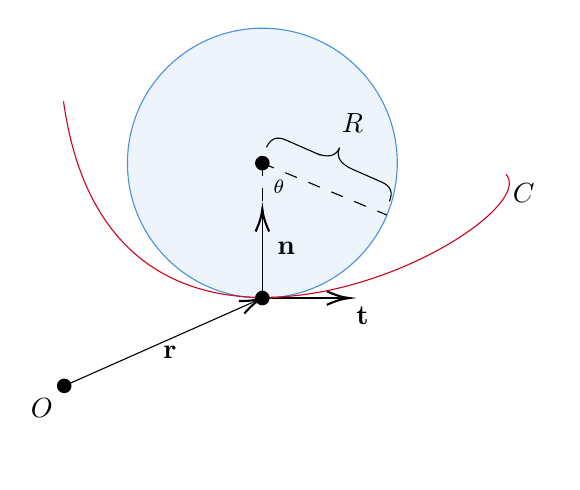
\begin{tikzpicture}[x=0.75pt,y=0.75pt,yscale=-1,xscale=1]
	%uncomment if require: \path (0,300); %set diagram left start at 0, and has height of 300
	
	%Shape: Ellipse [id:dp11623285715454001] 
	\draw  [draw opacity=0][fill={rgb, 255:red, 0; green, 0; blue, 0 }  ,fill opacity=1 ] (161.04,202.31) .. controls (161.04,200.37) and (162.61,198.8) .. (164.54,198.8) .. controls (166.48,198.8) and (168.05,200.37) .. (168.05,202.31) .. controls (168.05,204.24) and (166.48,205.81) .. (164.54,205.81) .. controls (162.61,205.81) and (161.04,204.24) .. (161.04,202.31) -- cycle ;
	%Straight Lines [id:da2508934300022321] 
	\draw    (164.54,202.31) -- (258.17,160.81) ;
	\draw [shift={(260,160)}, rotate = 516.1] [color={rgb, 255:red, 0; green, 0; blue, 0 }  ][line width=0.75]    (10.93,-3.29) .. controls (6.95,-1.4) and (3.31,-0.3) .. (0,0) .. controls (3.31,0.3) and (6.95,1.4) .. (10.93,3.29)   ;
	%Straight Lines [id:da7674997790762081] 
	\draw [color={rgb, 255:red, 0; green, 0; blue, 0 }  ,draw opacity=1 ]   (260,160) -- (300,160) ;
	\draw [shift={(302,160)}, rotate = 180] [color={rgb, 255:red, 0; green, 0; blue, 0 }  ,draw opacity=1 ][line width=0.75]    (10.93,-3.29) .. controls (6.95,-1.4) and (3.31,-0.3) .. (0,0) .. controls (3.31,0.3) and (6.95,1.4) .. (10.93,3.29)   ;
	%Shape: Circle [id:dp6348939130079169] 
	\draw  [color={rgb, 255:red, 74; green, 144; blue, 226 }  ,draw opacity=1 ][fill={rgb, 255:red, 74; green, 144; blue, 226 }  ,fill opacity=0.1 ] (195,95) .. controls (195,59.1) and (224.1,30) .. (260,30) .. controls (295.9,30) and (325,59.1) .. (325,95) .. controls (325,130.9) and (295.9,160) .. (260,160) .. controls (224.1,160) and (195,130.9) .. (195,95) -- cycle ;
	%Straight Lines [id:da4205464127260875] 
	\draw [draw opacity=0]   (260,95) -- (260,160) ;
	\draw [shift={(260,160)}, rotate = 90] [draw opacity=0][line width=0.75]      (0, 0) circle [x radius= 3.35, y radius= 3.35]   ;
	\draw [shift={(260,95)}, rotate = 90] [draw opacity=0][line width=0.75]      (0, 0) circle [x radius= 3.35, y radius= 3.35]   ;
	%Straight Lines [id:da5779811168879634] 
	\draw  [dash pattern={on 4.5pt off 4.5pt}]  (260,95) -- (320,120) ;
	%Straight Lines [id:da25785735111397157] 
	\draw [color={rgb, 255:red, 0; green, 0; blue, 0 }  ,draw opacity=1 ]   (260,160) -- (260,119) ;
	\draw [shift={(260,117)}, rotate = 450] [color={rgb, 255:red, 0; green, 0; blue, 0 }  ,draw opacity=1 ][line width=0.75]    (10.93,-3.29) .. controls (6.95,-1.4) and (3.31,-0.3) .. (0,0) .. controls (3.31,0.3) and (6.95,1.4) .. (10.93,3.29)   ;
	%Shape: Ellipse [id:dp504146351430413] 
	\draw  [draw opacity=0][fill={rgb, 255:red, 0; green, 0; blue, 0 }  ,fill opacity=1 ] (256.49,95) .. controls (256.49,93.06) and (258.06,91.49) .. (260,91.49) .. controls (261.94,91.49) and (263.51,93.06) .. (263.51,95) .. controls (263.51,96.94) and (261.94,98.51) .. (260,98.51) .. controls (258.06,98.51) and (256.49,96.94) .. (256.49,95) -- cycle ;
	%Curve Lines [id:da3234174981600959] 
	\draw [color={rgb, 255:red, 208; green, 2; blue, 27 }  ,draw opacity=1 ]   (164.2,65.2) .. controls (188.2,238.8) and (399.4,124.8) .. (377.4,100.4) ;
	%Shape: Ellipse [id:dp9921539771179669] 
	\draw  [draw opacity=0][fill={rgb, 255:red, 0; green, 0; blue, 0 }  ,fill opacity=1 ] (256.49,160) .. controls (256.49,158.06) and (258.06,156.49) .. (260,156.49) .. controls (261.94,156.49) and (263.51,158.06) .. (263.51,160) .. controls (263.51,161.94) and (261.94,163.51) .. (260,163.51) .. controls (258.06,163.51) and (256.49,161.94) .. (256.49,160) -- cycle ;
	%Shape: Brace [id:dp6625426388074377] 
	\draw   (321.2,113.4) .. controls (323.07,109.13) and (321.88,106.05) .. (317.61,104.18) -- (303.57,98.01) .. controls (297.46,95.33) and (295.35,91.85) .. (297.23,87.58) .. controls (295.35,91.85) and (291.36,92.65) .. (285.26,89.97)(288.01,91.18) -- (271.22,83.81) .. controls (266.95,81.93) and (263.87,83.13) .. (262,87.4) ;
	%Straight Lines [id:da3029069687640311] 
	\draw  [dash pattern={on 4.5pt off 4.5pt}]  (260,95) -- (260,117) ;
	
	% Text Node
	\draw (379.4,103.4) node [anchor=north west][inner sep=0.75pt]    {$C$};
	% Text Node
	\draw (147.2,207.2) node [anchor=north west][inner sep=0.75pt]    {$O$};
	% Text Node
	\draw (211,182) node [anchor=north west][inner sep=0.75pt]    {$\mathbf{r}$};
	% Text Node
	\draw (304,163) node [anchor=north west][inner sep=0.75pt]  [color={rgb, 255:red, 0; green, 0; blue, 0 }  ,opacity=1 ]  {$\mathbf{t}$};
	% Text Node
	\draw (264,102) node [anchor=north west][inner sep=0.75pt]  [font=\scriptsize]  {$\theta $};
	% Text Node
	\draw (266,132) node [anchor=north west][inner sep=0.75pt]  [color={rgb, 255:red, 0; green, 0; blue, 0 }  ,opacity=1 ]  {$\mathbf{n}$};
	% Text Node
	\draw (297,70) node [anchor=north west][inner sep=0.75pt]    {$R$};
	
	
	\end{tikzpicture}
	

\end{center}
A point on this circle can be described by
$$
\vv{x}(\theta) = \vv{r} + R(1 - \cos \theta) \vv{n} + R \sin \theta \vv{t}.
$$
Then expanding for $|\theta|$ small, we get
$$
\vv{x} (\theta) = \vv{r} + R \theta \vv{t} + \frac{1}{2} R \theta^2 \vv{n} + o(\theta^2).
$$
On this circle, the arc-length is $s = R \theta$. Thus if we express the above in terms of arc-length, we get
$$
\vv{x}(\theta) = \vv{r} + S \vv{t} + \frac{1}{2R} s^2 \vv{n} + o(s^2).
$$
As we want this to match the curve, we compare it to the equation for the curve near $\vv{r}$, and to match quadratic terms we need
$R = 1/\kappa$.

\begin{definition}[Radius of Curvature]
	We define $R(s)=1/\kappa(s)$ to be the \vocab{radius of curvature} of the curve $s \mapsto \vv{r}(s)$.
\end{definition}

\chapter{Coordinates, Differentials and Gradients}

\section{Differentials and First Order Changes}



\end{document}
